\chapter{Sensors}\label{chap:sensors}
Robots are systems that sense, actuate, and compute. So far, we have studied the basic physical principles of actuation, i.e., locomotion and manipulation, and computation, i.e., inverse kinematics and path-planning. We now need to understand the basic principles of robotic sensors that provide the data-basis for computation.

The goals of this chapter are
\begin{itemize}
\item provide an overview of sensors commonly used on robotic systems
\item outline the physical principles that are responsible for uncertainty in sensor-based reasoning
\end{itemize}

\section{Robotic Sensors}
The development of sensors is classically driven by industries other than robotics. These include submarines, automatically opening doors, safety devices for industry, servos for remote-controlled toys, and more recently the cell-phone, automobiles and gaming consoles. These industries are mostly responsible for making ``exotic'' sensors available at low cost by identifying mass-market applications, e.g., accelerometers and gyroscopes now being used in mass-market smart phones or the 3D depth sensor ``Kinect'' as part of its XBox gaming console.
\begin{framed}
Recap the sensors that you are interacting with daily. What sensors do you have in your phone, in your house and kitchen, or in your car?
\end{framed}
As we will see later on, sensors are hard to classify by their application. In fact, most problems benefit from every possible source of information that they can obtain. For example, localization can be achieved by counting encoder increments, but also by measuring acceleration, or using vision. All of these approaches differ drastically in their precision and the kind of data that they provide, but none of them is able to completely solve the localization problem on its own.
This chapter is therefore organized by the physical quantities (and derivatives thereof), a sensor is measuring, instead of the higher level state estimates it can contribute to.

\begin{framed}
Think about the kind of data that you could obtain from an encoder, an accelerometer, or a vision sensor on a non-holonomic robot. What are the fundamental differences?
\end{framed}
Although an encoder is able to measure position, it is used in this function only on robotic arms. If the robot is non-holonomic, closed tours in its configuration space, i.e., robot motions that return the encoder values to their initial position, do not necessarily drive the robot back to its starting point. In those robots, encoders are therefore mainly useful to measure speed. An accelerometer instead, by definition, measures the derivative of speed. Vision, finally, allows to calculate the absolute position (or the integral of speed) if the environment is equipped with unique features. An additional fundamental difference between those three sensors is the amount and kind of data they provide. An accelerometer samples real-valued quantities that are digitized with some precision. An odometer instead delivers discrete values that correspond to encoder increments. Finally, a vision sensor delivers an array of digitized real-valued quantities (namely colors). Although the information content of this sensor exceeds that of the other sensors by far, cherry-picking the information that are really useful remains a hard, and largely unsolved, problem.


\section{Proprioception of robot kinematics and internal forces}
\emph{Proprioception} \index{Proprioception} refers to the perception of internal states of a robot.
This is different from \emph{exteroception}\index{Exteroception}, which describes sensing of anything outside of the robot. Proprioception includes awareness of the robot's joint angles, its speeds, as well torques and forces.

The main internal sensor is therefore the encoder. Encoders can be used for sensing joint position and speed, as well as --- when used together with a spring --- a simple force sensor. There are both incremental and absolute encoders. The latter are mostly used in industrial applications, but are not common in mobile robotics. There are magnetical and optical encoders, which both rely on a magnetic or optical beacon turning together with the motor and being sensed by an appropriate sensor that counts every pass-through. The most common encoder in robotics is the optical \emph{quadrature encoder} \index{Quadrature encoder}. It relies on a pattern rotating with the motor and an optical sensor that can register black/white transitions. Whereas those patterns can be precision manufactured, simple encoders can be made by simply laser-cutting a pattern such as shown in Figure~\ref{fig:encoders} and reading it with a light sensor.

\begin{figure}
	\centering
		\includegraphics[width=0.3\textwidth]{figs/encoderdisk.png}
		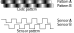
\includegraphics[width=0.3\textwidth]{figs/quadraturencoder.png}
		\includegraphics[width=0.3\textwidth]{figs/absoluteencoder.png}
	\caption{From left to right: encoder pattern used in a quadrature encoder, resulting sensor signal (forward motion), absolute encoder pattern (gray coding).}
	\label{fig:encoders}
\end{figure}

While a single sensor would be sufficient to detect rotation and its speed, it does not allow for the determining the direction of motion. Quadrature encoders therefore have two sensors, A and B, that register an interleaving pattern with distance of a quarter phase. If A leads B, for example, the disk is rotating in a clockwise direction. If B leads A, then the disk is rotating in a counter-clockwise direction. It is also possible to create absolute encoders, an example of which is shown in Figure~\ref{fig:encoders}, right. This pattern encodes 3-bits, encoding 8 different segments on a disc. Notice that the pattern is arranged in such a way that there is only one bit changing from one segment to the other. This is known as ``Gray code''\index{Gray code}. The function of linear encoders is analogous, both for incremental and absolute encoders.

If combined with a spring, such as in a series elastic actuator, rotary and linear encoders can be used as simple force/torque sensors using Hooke's law ($F=kx$, force equals distance times spring constant). Whereas the series elastic actuator is the most illustrative examples, most load cells operate on the premise of measuring displacements within materials of known properties. Here, measuring changes in resistance or capacitance might be easier choices.

Other means of measuring the actual force at the end-effector or joint torques is measuring the actual current consumed at each joint. Knowing a mechanism's pose allows to calculate the resulting forces and torques across the mechanism as well as the currents required for empty loading conditions. Derivations of these then correspond to additional forces that can hence be calculated.

Finally, there are other means of proprioception, such as simple sensors that can detect when a robot gets picked up, e.g.

\section{Sensors using light}
The small form factor and low price of light-sensitive semi-conductors have led to a proliferation of light-based sensing relying on a multitude of physical effects. These include reflection, phase shift, and time of flight.

\subsection{Reflection}
Reflection is one of the principles that is easiest to exploit: the closer an object is, the more it reflects light shined at it. This allows to easily measure distance to objects that reflect light well and are not too far away. In order to make these sensors as independent from an object's color (but unfortunately not totally independent), infrared is most commonly chosen. A distance sensor is made from two components: an emitter and a receiver. They work by emitting an infrared signal and then measuring the strength of the reflected signal. A typical response is shown in Figure~\ref{fig:epuckir}. The values obtained at an analog-digital converter correspond to the voltage at the infrared receiver and are saturated for low distances (flat line), and quadratically fall off thereafter.

\begin{figure}
	\centering
		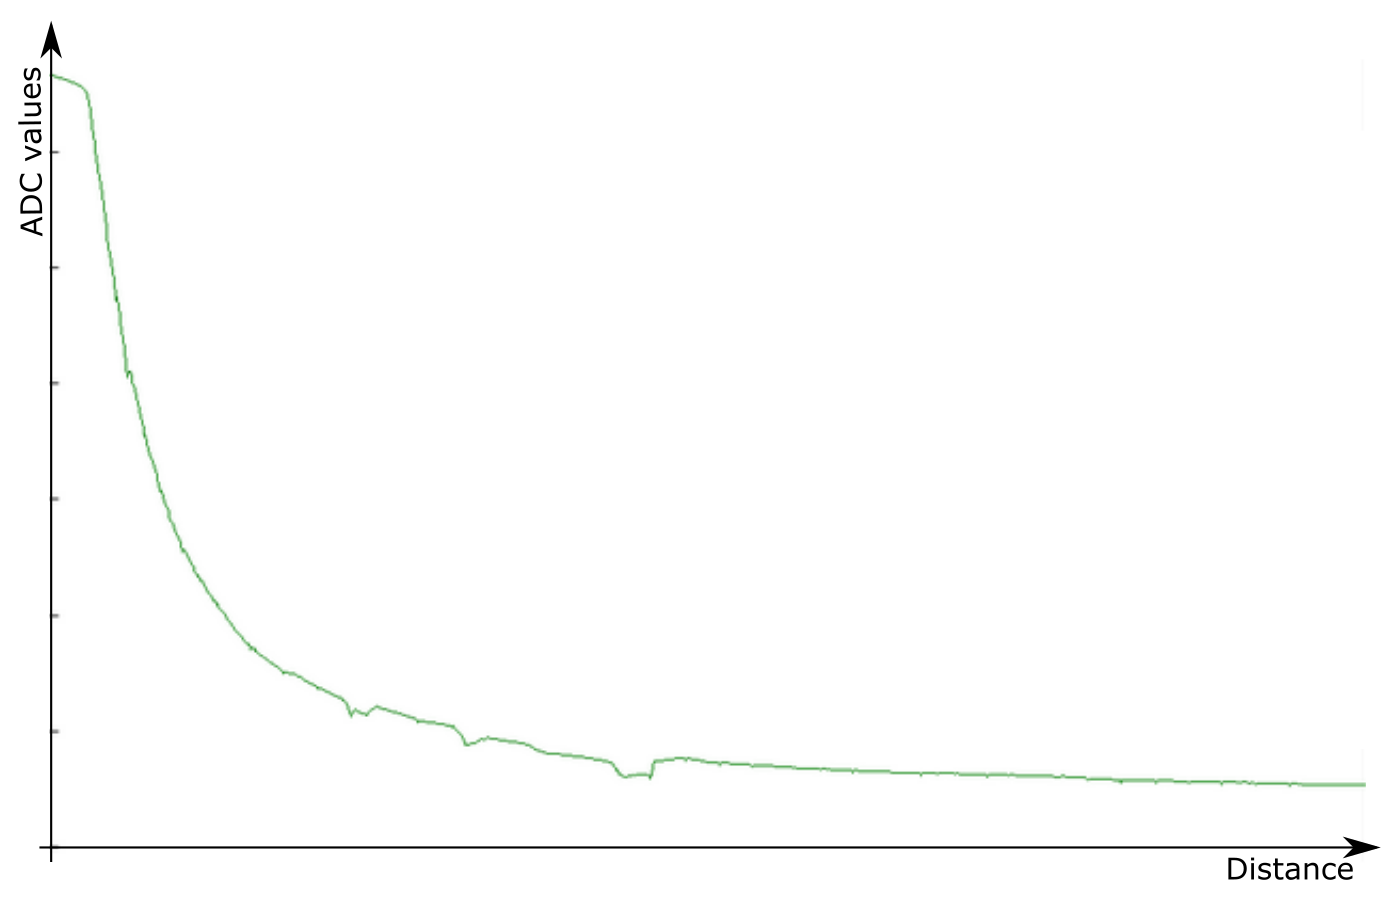
\includegraphics[width=0.8\textwidth]{figs/epuckirsensor.png}
	\caption{Typical response of an infrared distance sensor as a function of distance. Units are left dimensionless intensionally.}
	\label{fig:epuckir}
\end{figure}

When using more than one infrared sensor/emitter pair, e.g., using a camera and a projector not only allows to measure the distance of many points at once, but also to assess the structure of the environment by calculating its impact on the deformation of patterns. For example a straight line becomes a curve when projected onto a round surface. This approach is known as \emph{structured light}\index{Structured light} and illustrated in Figure~\ref{fig:struclight}. Thanks to the continuously increasing efficiency of computational systems, a light-weight version of such an approach has become feasible to be implemented at small scale and low cost at around 2010, and emerged as a novel standard in robotic sensing.

\begin{figure}
	\centering
		\includegraphics[width=\textwidth]{figs/structuredlight.png}
	\caption{From left to right: two complex physical objects, a pattern of colored straight lines and their deformation when hitting the surfaces, reconstructed 3D shape. From \protect\cite{zhang2002rapid}.}
	\label{fig:struclight}
\end{figure}

Instead of using line patterns, infrared-based depth image sensors use a speckle pattern (a collection of randomly distributed dots with varying distances), and two computer vision concepts: \emph{depth from focus} and \emph{depth from stereo}.\index{Depth from Focus}\index{Depth from Stereo} When using a lens with a narrow focal depth, objects that are closer or farther away appear blurred (you can easily observe this on professional portrait photos, which often use this effect for aesthetic purposes). Measuring the ``bluriness'' of a scene (for known camera parameters) therefore allows for an initial estimate of depth. Depth from stereo instead works by measuring the disparity of the same object appearing in two images taken by cameras that are a known distance apart. Being able to identify the same object in both frames allows to calculate this disparity, and from there the distance of the object. (The farther the object is away, the smaller is the disparity.) This is where the speckle pattern comes in handy, which simply requires to search for blobs with similar size that are close to each other.


\subsection{Phase shift}\label{sec:phaseshiftsensors}
As you can see in Figure~\ref{fig:epuckir}, reflection can only be precise if distances are short. Instead of measuring the strength (aka amplitude) of the reflected signal, laser distance sensors measure the phase difference of the reflected wave. In order to do this, the emitted light is modulated with a wave-length that exceeds the maximum distance the scanner can measure. If you would use visible light and do this much slower, you would see a light that keeps getting brighter, then getting darker, briefly turns off and then starts getting brighter again. Thus, if you would plot the amplitude, i.e.\ its brightness, of the emitted signal vs.\ time you would see a wave that has zero-crossings when the light is dark. As light travels with the speed of light, this wave propagates through space with a constant distance (the wavelength) between its zero crossings. When it gets reflected, the same wave travels back (or at least parts of it that get scattered right back). For example, modern laser scanners\index{Laser range finder} emit signals with a frequency of 5 MHz (turning off 5 million times in one second). Together with the speed of light of approximately 300,000km/s, this leads to a wavelength of 60m and makes such a laser scanner useful up to 30m.

When the laser is now at a distance that corresponds exactly to one half the wave-length, the reflected signal it measures will be dark at the exact same time its emitted wave goes through a zero-crossing. Going closer to the obstacle results in an offset that can be measured. As the emitter knows the shape of the wave it emitted, it can calculate the phase difference between emitted and received signal. Knowing the wave-length it can now calculate the distance. As this process is independent from ambient light (unless it has the exact same frequency as the laser being used), the estimates can be very precise. This is in contrast to a sensor that uses signal strength. As the signal strength decays at least quadratically, small errors, e.g.\ due to fluctuations in the power supply that drives the emitting light, noise in the analog-digital converter, or simply differences in the reflecting surface have drastic impact on the accuracy and precision (see below for a more formal definition of this term).

As the laser distance measurement process is fast, such lasers can be combined with rotating mirrors to sweep larger areas, known as \emph{Laser Range Scanners}\index{Laser Range Scanners}. Such systems have been combined into packages consisting of up to 64 scanning lasers, providing a depth map around a car while driving, e.g.\ It is also possible to modulate projected images with a phase-changing signal, which is the operational principle of early ``time-of-flight'' cameras, which is not an accurate description of their operation, however

\subsection{Time-of-flight}
The most precise distance measurements light can provide is by measuring its time of flight. This can be done by counting the time a signal from the emitter becomes visible in the receiver. As light travels very fast (3,000,000,000m/s), this requires high-speed electronics that can measure time periods smaller than nano-seconds in order to achieve centimeter accuracy. In practice this is done by combining the receiver with a very fast (electronic) shutter that operates at the same frequency with which light is emitted. As this timing is known, one can infer the time light must have been traveling by measuring the quantity of photons that have made it back from the reflective surface within one shutter period. Considering a concrete example, light travels 15m in 50ns. Therefore, it will take a pulse 50ns to return from an object at a distance of 7.5m. If the camera sends out a pulse of 50ns length and then closes the receiver with a shutter, the receiver will receive more photons the closer the object is, but no photons if the object is farther away than 7.5m. Given a fast enough and precise circuit that acts as a shutter, it is sufficient to measure the actual amount of light that returns from the emitter.

\section{Sensors using sound}
\subsection{Ultra-sound distance sensors}
Ultra-sound distance sensor: An ultra-sound distance sensor operates by emitting an ultra-sound pulse and measures its reflection. Unlike a light-based sensor that measures the amplitude of the reflected signal, a sound-based sensor measures the time it took the sound to travel. This is possible, because sound travels at much lower speed (300m/s) than light (300,000km/s). The fact that the sensor actually has to wait for the signal to return leads to a trade-off between range and bandwidth. (Look these definitions up above before you read on.) In other words, allowing a longer range requires waiting longer, which in turn limits how often the sensor can provide a measurement. Although US distance sensors have become less and less common in robotics, they have an advantage over light-based sensors: instead of sending out a ray, the ultra-sound pulse results in a cone with an opening angle of 20 to 40 degrees. By this, US sensors are able to detect small obstacles without the requirement of directly hitting them with a ray. This property makes them the sensor of choice in automated parking helpers in cars.

\subsection{Texture recognition}
Audible sound consists of high frequency vibrations in the range between 20 Hz and roughly 15 kHz. Microphones are therefore ideally suited to measure vibrations in this range. This allows them to double as the Pascinian corpuscle in human skin cells, which is known to have a resonance frequency of 250 Hz and is mostly responsible for texture recognition. Indeed, rubbing a texture against a microphone can indeed be used for differentiating between tens and hundreds of different textures \cite{hughes14}, with a number of commercial sensors available. These sensors usually calculate the frequency spectrum of the recorded signal, which can then be classified using machine learning techniques. Being able to recognize a texture by touch is important in applications like grasping and navigation through cluttered terrain.

\section{Inertia-based sensors}
A moving mass does not loose its kinetic energy, but for friction. Likewise, a resting mass will resist acceleration. Both effects are due to ``inertia'' \index{Inertia} and can be exploited to measure acceleration and speed.

\subsection{Accelerometer}
An accelerometer \index{Accelerometer}can be thought of as a mass on a dampened spring. Considering a vertical spring with a mass hanging down from it, we can measure the acting force $F=kx$ (Hooke's law) \index{Hooke's law}by measuring the displacement $x$ that the mass has stretched the spring. Using the relationship $F=am$, we can now calculate the acceleration $a$ on the mass $m$. On earth, this acceleration is roughly $9.81\frac{kg m}{s^2}$. In practice, these spring/mass systems are realized using microelectromechanical systems (MEMS), such as a cantilevered beam whose displacement can be measured, e.g., using a capacitive sensor. Accelerometers measure up to three axes of translational accelerations. Infering a position from this requires integration twice, thereby amplifying any noise, making position estimates using accelerometers alone infeasible. As gravity provides a constant acceleration vector, accelerometers are very good at estimating the pose of an object with respect to gravity.

\subsection{Gyroscopes}
A gyroscope is an electro-mechanical device that can measure rotational orientation. It is complementary to the accelerometer that measures translational acceleration. Classically, a gyroscope consists of a rotating disc that could freely rotate in a system of pivots and gimbals. When moving the system, the inertial momentum keeps the original orientation of the disc, allowing to measure the orientation of the system relative to where the system was started. A variation of the gyroscope is the rate gyro, which measures rotational speed.

What a rate gyro \index{Rate gyro}\index{Gyroscopes} measures can most intuitively be illustrated by considering the implementation of an \emph{optical} rate gyro. In an optical gyro, a laser beam is split into two beams and send around a circular path in two opposite directions. If this setup is rotated against the direction of one of these laser beams, one laser will have to travel slightly longer than the other, leading to a measurable phase-shift at the receptor. This phase shift is proportional to the \emph{rotational speed} of the setup. As light with the same frequency and phase will add, and lights with the same frequency but opposite phases will cancel each other, light at the detector will be darker for high rotational velocities. As small-scale optical rate gyros are not practical for multiple reasons, MEMS rate gyros rely on a mass suspended by springs. The mass is actively vibrating, making it subject to Coriolis forces, when the sensor is rotated. Coriolis forces can be best understand by moving orthogonally to the direction of rotation on a vinyl disk player. In order to move in a straight line, you will not only need to move forwards, but also sideways. The necessary acceleration to change the speed of this sideway motion is counteracting the Coriolis force, which is both proportional to the lateral speed (the vibration of the mass in a MEMS sensor) and the rotational velocity, which the device wishes to measure. Note that the MEMS gyro would only be able to measure acceleration if it were not vibrating.

Gyroscopes can measure the rotational speed around three axes, which can be integrated to obtain absolute orientation. As an accelerometer measures along three axes of translation, the combination of both sensors can provide information on motion in all six degrees of freedom. Together with a magnetometer (compass), which provides absolute orientation, this combination is also known as \emph{Inertial Measurement Unit} (IMU), \index{Inertial Measurement Unit}\index{IMU}.

\section{Beacon-based sensors}
Localizing an object by triangulation goes back to ancient civilizations orienting themselves using the stars. As stars are only visible during unclouded nights, seafarers have eventually invented systems of artificial beacons emitting light, sound, and eventually radio waves. The most sophisticated of such systems is the Global Positioning System (GPS). GPS consists of a number of satellites in orbit, which are equipped with knowledge about their precise location and have synchronized clocks. These satellites broadcast a radio signal that travels at the speed of light and is coded with its time of emission. GPS receivers can therefore calculate the distance to each satellite by comparing time of emission and time of arrival. As not only the position (x,y,z), but also the time difference between the GPS receiver's clock and the synchronized clocks of the satellites is unknown, four satellites are needed to obtain a ``fix''. Due to the way information from the satellites is coded, getting an initial fix can take in the order of minutes, but eventually is available multiple times a second. GPS measurements are neither precise nor accurate enough (see below) for small mobile robots, and require to be combined with other sensors, such as IMUs and compasses. (The bearing shown on some GPS receivers is calculated from subsequent positions and is therefore meaningless if the robot is not moving.)

There exist also a variety of indoor-GPS solutions, which consists of either active or passive beacons that are mounted in the environment at known locations. Passive beacons, for example infrared reflecting stickers arranged in a certain pattern or 2D barcodes, can be detected using cameras and their pose can be calculated from their known dimensions. Active beacons instead usually emit radio, ultrasound or a combination thereof, which can then be used to estimate the robot's range to this beacon.

\section{Terminology}
It is now time to introduce  a more precise definition of terms such as ``speed'' and ``resolution", as well as additional taxonomy that is used in a robotic context. %Roboticists differentiate between proprioceptive and exteroceptive sensors. Proprioceptive sensors measure quantities that are internal to the robot such as wheel-speed, current consumption, joint position or battery status. Exteroceptive sensors measure quantities from the environment, such as distance to a wall, the strength of ambient light or the pattern of a picture at the wall.

Roboticists differentiate between \emph{active} and \emph{passive} sensors. Active sensors \index{Active sensor} emit energy of some sort and measure the reaction of the environment. Passive sensors \index{Passive sensor} instead measure energy from the environment. For example, most distance sensors are active sensors (as they sense the reflection of a signal they emit), whereas an accelerometer, compass, or a push-button are passive sensors.

The difference between the upper and the lower limit of the quantity a sensor can measure its known as its \emph{range}~\index{Range (sensor)}. This should not be confused with the \index{Dynamic Range (sensor)} \emph{dynamic range}, which is the ratio between the highest and lowest value a sensor can measure. It is usually expressed on a logarithmic scale (to the basis 10), also known as ``decibel''\index{Decibel}. The minimal distance between two values a sensor can measure is known as its \index{Resolution (sensor)} \emph{resolution}. The resolution of a sensor is given by the device physics (e.g., a light detector can only count multiples of a quant), but usually limited by the analog-digital conversion process. The resolution of a sensor should not be confused with its accuracy or its precision (which are two different concepts). For example, whereas an infrared distance sensor might yield 4096 different values to encode distances from 0 to 10cm, which suggests a resolution of around 24 micrometers, its precision is far above that (in the order of millimeters) due to noise in the acquisition process.

Technically, a sensors accuracy \index{Accuracy (sensor)} is given by the difference between a sensors (average) output $m$ and the true value $v$:
\begin{equation}
accuracy=1-\frac{|m-v|}{v}
\end{equation}
This measure provides you with a quantity that approaches one for very accurate values and zero if the measurements group far away from the actual mean. In practice, however, this measure is only rarely used and accuracy is provided with absolute values or a percentage at which a value might exceed the true measurement.

A sensor's precision \index{Precision (sensor)} instead is given by the ratio of range and statistical variance of the signal. Precision is therefore a measure of repeatability of a signal, whereas accuracy describes a systematic error that is introduced by the sensor physics. This is illustrated in Figure~\ref{fig:precision}.
\begin{figure}
	\centering
		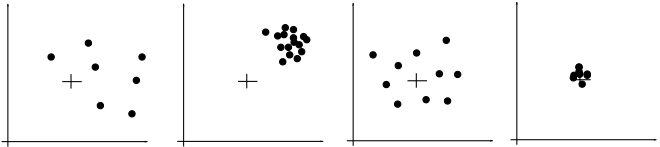
\includegraphics[width=0.9\textwidth]{figs/precisionvsaccuracy.png}
	\caption{From left to right, the cross corresponds to the true value of the signal: neither precise nor accurate, precise but not accurate, accurate but not precise, accurate and precise.
	\label{fig:precision}}
\end{figure}

A GPS sensor is usually precise within a few meters, but only accurate to tens of meters. This becomes most obvious when satellite configurations change, resulting in the precise region jumping by a couple of meters. In practice, this can be avoided by fusing this data with other sensors, e.g.\ from an IMU.

The speed at which a sensor can provide measurements is known as its \index{Bandwidth (sensor)} \emph{bandwidth}. For example, if a sensor has a bandwidth of 10 Hz, it will provide a signal ten times a second. This is important to know, as querying the sensor more often is a waste of computational time and potentially misleading.


\section*{Take-home lessons}
\begin{itemize}
\item Most of a robot's sensors either address the problem of robot localization or localizing and recognizing objects in its vicinity.
\item Each sensors has advantages and drawbacks that are quantified in its range, precision, accuracy, and bandwidth. Therefore, robust solutions to a problem can only be achieved by combining multiple sensors with differing operation principles.
\item Solid-state sensors (i.e.\ without mechanical parts) can be miniaturized and cheaply manufactured in quantity. This has enabled a series of affordable IMUs and 3D depth sensors that will provide the data basis for localization and object recognition on mass-market robotic systems.
\end{itemize}

\section*{Exercises}\small
\begin{enumerate}
\item Given a laser scanner with an angular resolution of 0.01 rad and a maximum range of 5.6 meters, what is the minimum range $d$ a robot needs to have from an object of 1cm width to definitely sense it, i.e., hit it with at least one of its rays? You can approximate the distance between two rays with the arc length.
\item Why does the bandwidth of a Ultra-sound based distance sensor decreases significantly when increasing its dynamic range, but that of a laser range scanner does not for typical operation?
\item You are designing an autonomous electric car to transport goods on campus. As you are worried about cost, you are thinking about whether to use a laser scanner or an ultra-sound sensor for detecting obstacles. As you drive rather slow, you are required to sense up to 15 meters. The laser scanner you are considering can sense up to this range and has a bandwidth of 10Hz. Assume 300m/s for the speed of sound in the following.
\begin{enumerate}
\item Calculate the time it takes until you hear back from the US sensor when detecting an obstacle 15m away. Assume that the robot is not moving at this point.
\item Calculate the time it takes until you hear back from the laser scanner. Hint: you don’t need the speed of light for this, the answer is in the specs above.
\item Assume now that you are moving toward the obstacle. Which sensor will give you a measurement that is closer to your real distance at the time of reading and why?
\end{enumerate}
\end{enumerate}\normalsize
